
For Frame Error Rate we have de following graph:
\begin{figure}[!htbp]
	\centering
	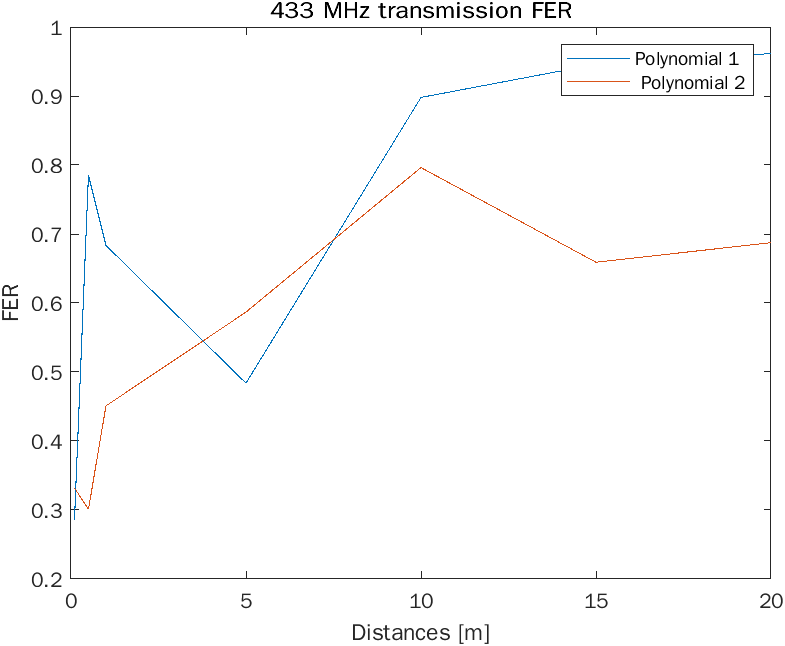
\includegraphics [width=9.5cm]{images/FERt.png}
	\caption{FER graph}
\end{figure} 

We can observe that as the distance increases, the FER also increases, this is because less packets arrive and most of them were incorrect.

The values taken were:


	\begin{table} [!htbp]
		\centering
		\caption{FER values}
			\shadowbox{
			\begin{tabular}{|c|c|c|}
			\hline
			\textbf{Distance} & Polynomial 1 & Polynomial 2 \\ \hline
			10 cm    &  	0.2857   & 0.3320    \\
			50 cm  &  0.7849  & 0.3011 \\
			1 m  & 0.6835  & 0.4510 \\
			5 m  & 0.4839 &  0.5869 \\
			10 m  &  0.8980 &  0.7963 \\
			25 m  & 0.9459  & 0.6591\\
			20 m &  0.9615 &     0.6875 \\ \hline
		\end{tabular}
	}
	\end{table}

